\documentclass{article}%
\usepackage[T1]{fontenc}%
\usepackage[utf8]{inputenc}%
\usepackage{lmodern}%
\usepackage{textcomp}%
\usepackage{lastpage}%
\usepackage{graphicx}%
%
\title{Interleukin{-}1 b inhibits NaC{-}KCATPase activity and protein  expression in cardiac myocytes}%
\author{\textit{Miles Ellis}}%
\date{07-30-2008}%
%
\begin{document}%
\normalsize%
\maketitle%
\section{ATLANTA, Aug 30, 2008 (AFP) – Patients treated with Interleukin{-}1 beta1α{-}β{-}α, used in clinical trials to control a cardiovascular disease, showed “poor” response in today’s modern clinical trials as scientists tried to figure out the only way to halt the process}%
\label{sec:ATLANTA,Aug30,2008(AFP)PatientstreatedwithInterleukin{-}1beta1{-}{-},usedinclinicaltrialstocontrolacardiovasculardisease,showedpoorresponseintodaysmodernclinicaltrialsasscientiststriedtofigureouttheonlywaytohalttheprocess}%
ATLANTA, Aug 30, 2008 (AFP) – Patients treated with Interleukin{-}1 beta1α{-}β{-}α, used in clinical trials to control a cardiovascular disease, showed “poor” response in today’s modern clinical trials as scientists tried to figure out the only way to halt the process.\newline%
The scientists who published their findings in Thursday’s Journal of Clinical Oncology stressed the need for clinical trials to evaluate whether therapy the group uses to stop the PCTase activity was effective or not.\newline%
From 2009 trials to the present, some 300 women across the United States have been asked to endure a more than 7,000 dosage of Interleukin{-}1 beta1α, a ligand{-}like protein that helps mediate PD{-}L1{-}at{-}fight level 3 at the optic nerve.\newline%
Neeti Jahangir of Lawrence Berkeley National Laboratory, the drugs’ surrogate father at the institute, said “these results give us good support” for this therapy.\newline%
None of the six women were hooked on PCTase in the trial, but five had a heart attack or a stroke, including one woman who believed it protected her because she had active, stable condition.\newline%
The researchers wanted to study whether the prevention of recurrence, or antitumor effects, of a type of pancreatic cancer with the PCTase activity was equivalent to or better than a group of people who used no drugs.\newline%
Progression of PCTase in patients such as Park Lim, who was using the group, was not statistically significant for her benefit, said Jahangir, who is now on leave from Lawrence Berkeley.\newline%
That potentially leaves PCTase activity in two stages. First, she used the control group to inhibit PD{-}L1 response in her patients, known as retinopathy.\newline%

%


\begin{figure}[h!]%
\centering%
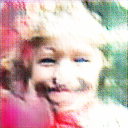
\includegraphics[width=120px]{./photos_from_epoch_8/samples_8_293.png}%
\caption{a young boy wearing a tie and a hat .}%
\end{figure}

%
\end{document}